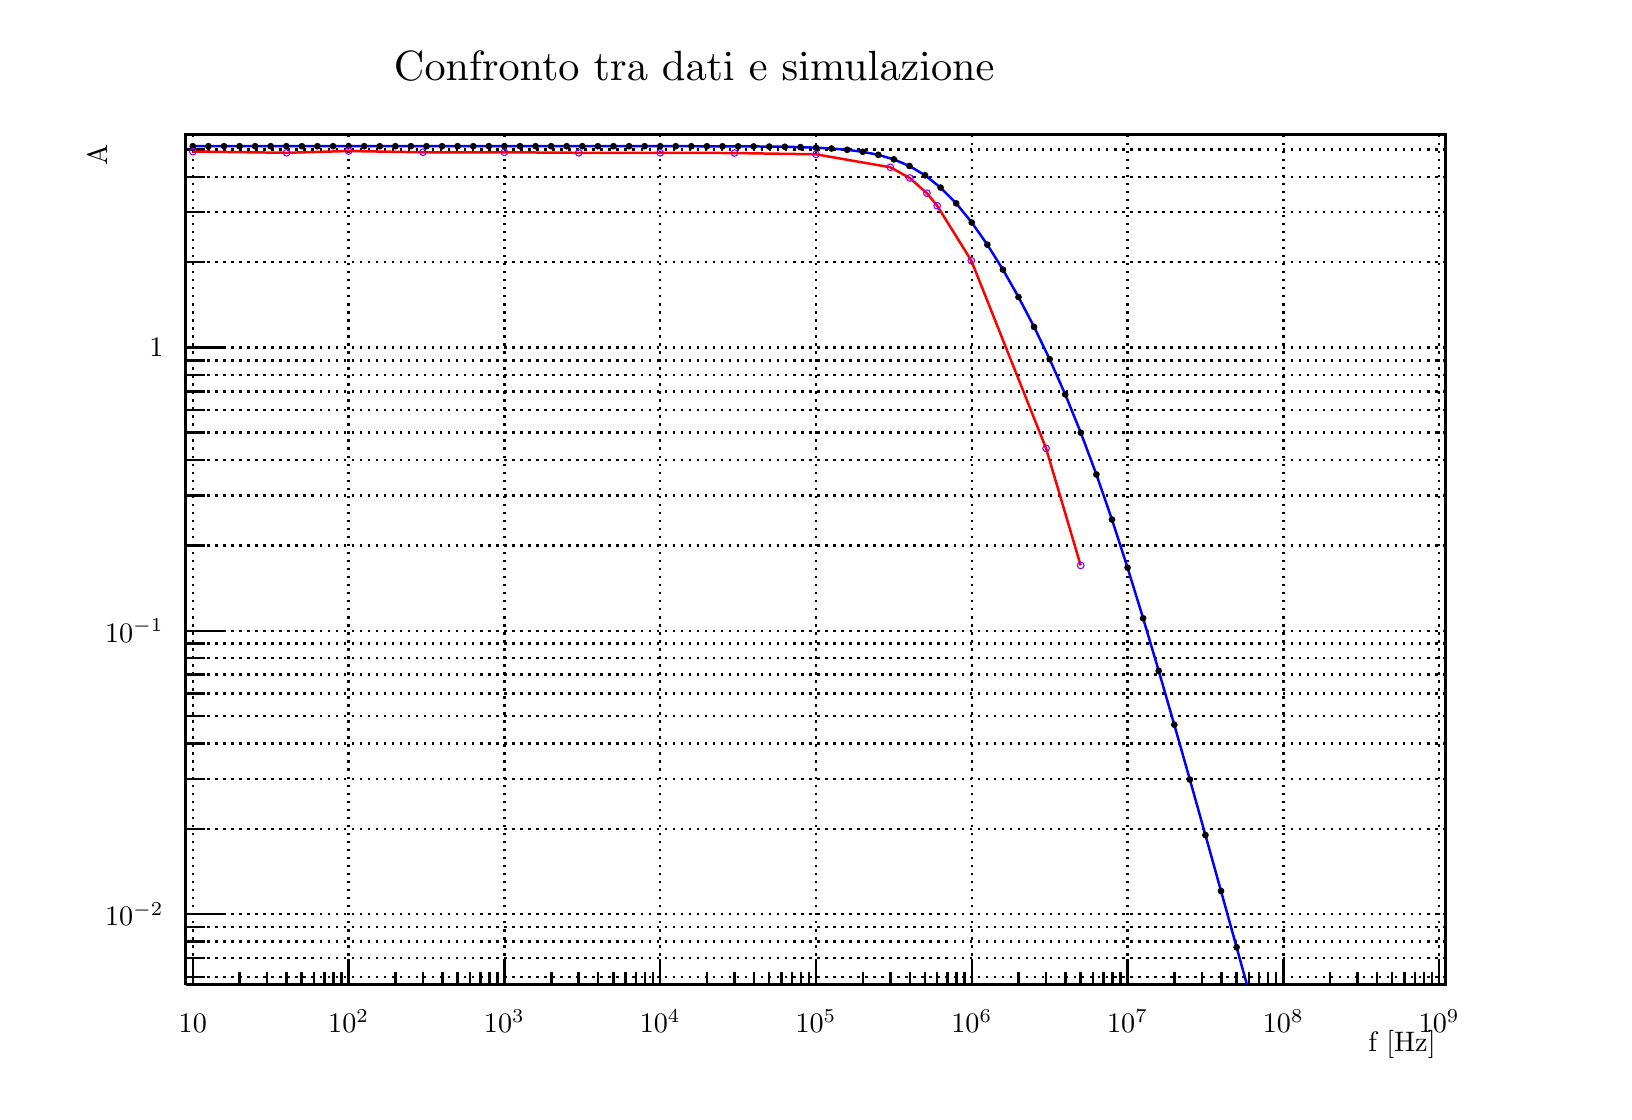
\begin{tikzpicture}
\pgfdeclareplotmark{cross} {
\pgfpathmoveto{\pgfpoint{-0.3\pgfplotmarksize}{\pgfplotmarksize}}
\pgfpathlineto{\pgfpoint{+0.3\pgfplotmarksize}{\pgfplotmarksize}}
\pgfpathlineto{\pgfpoint{+0.3\pgfplotmarksize}{0.3\pgfplotmarksize}}
\pgfpathlineto{\pgfpoint{+1\pgfplotmarksize}{0.3\pgfplotmarksize}}
\pgfpathlineto{\pgfpoint{+1\pgfplotmarksize}{-0.3\pgfplotmarksize}}
\pgfpathlineto{\pgfpoint{+0.3\pgfplotmarksize}{-0.3\pgfplotmarksize}}
\pgfpathlineto{\pgfpoint{+0.3\pgfplotmarksize}{-1.\pgfplotmarksize}}
\pgfpathlineto{\pgfpoint{-0.3\pgfplotmarksize}{-1.\pgfplotmarksize}}
\pgfpathlineto{\pgfpoint{-0.3\pgfplotmarksize}{-0.3\pgfplotmarksize}}
\pgfpathlineto{\pgfpoint{-1.\pgfplotmarksize}{-0.3\pgfplotmarksize}}
\pgfpathlineto{\pgfpoint{-1.\pgfplotmarksize}{0.3\pgfplotmarksize}}
\pgfpathlineto{\pgfpoint{-0.3\pgfplotmarksize}{0.3\pgfplotmarksize}}
\pgfpathclose
\pgfusepathqstroke
}
\pgfdeclareplotmark{cross*} {
\pgfpathmoveto{\pgfpoint{-0.3\pgfplotmarksize}{\pgfplotmarksize}}
\pgfpathlineto{\pgfpoint{+0.3\pgfplotmarksize}{\pgfplotmarksize}}
\pgfpathlineto{\pgfpoint{+0.3\pgfplotmarksize}{0.3\pgfplotmarksize}}
\pgfpathlineto{\pgfpoint{+1\pgfplotmarksize}{0.3\pgfplotmarksize}}
\pgfpathlineto{\pgfpoint{+1\pgfplotmarksize}{-0.3\pgfplotmarksize}}
\pgfpathlineto{\pgfpoint{+0.3\pgfplotmarksize}{-0.3\pgfplotmarksize}}
\pgfpathlineto{\pgfpoint{+0.3\pgfplotmarksize}{-1.\pgfplotmarksize}}
\pgfpathlineto{\pgfpoint{-0.3\pgfplotmarksize}{-1.\pgfplotmarksize}}
\pgfpathlineto{\pgfpoint{-0.3\pgfplotmarksize}{-0.3\pgfplotmarksize}}
\pgfpathlineto{\pgfpoint{-1.\pgfplotmarksize}{-0.3\pgfplotmarksize}}
\pgfpathlineto{\pgfpoint{-1.\pgfplotmarksize}{0.3\pgfplotmarksize}}
\pgfpathlineto{\pgfpoint{-0.3\pgfplotmarksize}{0.3\pgfplotmarksize}}
\pgfpathclose
\pgfusepathqfillstroke
}
\pgfdeclareplotmark{newstar} {
\pgfpathmoveto{\pgfqpoint{0pt}{\pgfplotmarksize}}
\pgfpathlineto{\pgfqpointpolar{44}{0.5\pgfplotmarksize}}
\pgfpathlineto{\pgfqpointpolar{18}{\pgfplotmarksize}}
\pgfpathlineto{\pgfqpointpolar{-20}{0.5\pgfplotmarksize}}
\pgfpathlineto{\pgfqpointpolar{-54}{\pgfplotmarksize}}
\pgfpathlineto{\pgfqpointpolar{-90}{0.5\pgfplotmarksize}}
\pgfpathlineto{\pgfqpointpolar{234}{\pgfplotmarksize}}
\pgfpathlineto{\pgfqpointpolar{198}{0.5\pgfplotmarksize}}
\pgfpathlineto{\pgfqpointpolar{162}{\pgfplotmarksize}}
\pgfpathlineto{\pgfqpointpolar{134}{0.5\pgfplotmarksize}}
\pgfpathclose
\pgfusepathqstroke
}
\pgfdeclareplotmark{newstar*} {
\pgfpathmoveto{\pgfqpoint{0pt}{\pgfplotmarksize}}
\pgfpathlineto{\pgfqpointpolar{44}{0.5\pgfplotmarksize}}
\pgfpathlineto{\pgfqpointpolar{18}{\pgfplotmarksize}}
\pgfpathlineto{\pgfqpointpolar{-20}{0.5\pgfplotmarksize}}
\pgfpathlineto{\pgfqpointpolar{-54}{\pgfplotmarksize}}
\pgfpathlineto{\pgfqpointpolar{-90}{0.5\pgfplotmarksize}}
\pgfpathlineto{\pgfqpointpolar{234}{\pgfplotmarksize}}
\pgfpathlineto{\pgfqpointpolar{198}{0.5\pgfplotmarksize}}
\pgfpathlineto{\pgfqpointpolar{162}{\pgfplotmarksize}}
\pgfpathlineto{\pgfqpointpolar{134}{0.5\pgfplotmarksize}}
\pgfpathclose
\pgfusepathqfillstroke
}
\definecolor{c}{rgb}{1,1,1};
\draw [color=c, fill=c] (0,0) rectangle (20,13.4957);
\draw [color=c, fill=c] (2,1.34957) rectangle (18,12.1461);
\definecolor{c}{rgb}{0,0,0};
\draw [c,line width=0.9] (2,1.34957) -- (2,12.1461) -- (18,12.1461) -- (18,1.34957) -- (2,1.34957);
\definecolor{c}{rgb}{1,1,1};
\draw [color=c, fill=c] (2,1.34957) rectangle (18,12.1461);
\definecolor{c}{rgb}{0,0,0};
\draw [c,line width=0.9] (2,1.34957) -- (2,12.1461) -- (18,12.1461) -- (18,1.34957) -- (2,1.34957);
\draw [c,line width=0.9] (2,1.34957) -- (18,1.34957);
\draw [c,dotted,line width=0.9] (2.09053,12.1461) -- (2.09053,1.34957);
\draw [c,dotted,line width=0.9] (4.06897,12.1461) -- (4.06897,1.34957);
\draw [c,dotted,line width=0.9] (6.04742,12.1461) -- (6.04742,1.34957);
\draw [c,dotted,line width=0.9] (8.02587,12.1461) -- (8.02587,1.34957);
\draw [c,dotted,line width=0.9] (10.0043,12.1461) -- (10.0043,1.34957);
\draw [c,dotted,line width=0.9] (11.9828,12.1461) -- (11.9828,1.34957);
\draw [c,dotted,line width=0.9] (13.9612,12.1461) -- (13.9612,1.34957);
\draw [c,dotted,line width=0.9] (15.9397,12.1461) -- (15.9397,1.34957);
\draw [c,dotted,line width=0.9] (17.9181,12.1461) -- (17.9181,1.34957);
\draw [c,line width=0.9] (2,1.34957) -- (2,12.1461);
\draw [c,dotted,line width=0.9] (18,1.44637) -- (2,1.44637);
\draw [c,dotted,line width=0.9] (18,1.68731) -- (2,1.68731);
\draw [c,dotted,line width=0.9] (18,1.89601) -- (2,1.89601);
\draw [c,dotted,line width=0.9] (18,2.0801) -- (2,2.0801);
\draw [c,dotted,line width=0.9] (18,2.24478) -- (2,2.24478);
\draw [c,dotted,line width=0.9] (18,3.32814) -- (2,3.32814);
\draw [c,dotted,line width=0.9] (18,3.96186) -- (2,3.96186);
\draw [c,dotted,line width=0.9] (18,4.4115) -- (2,4.4115);
\draw [c,dotted,line width=0.9] (18,4.76027) -- (2,4.76027);
\draw [c,dotted,line width=0.9] (18,5.04523) -- (2,5.04523);
\draw [c,dotted,line width=0.9] (18,5.28616) -- (2,5.28616);
\draw [c,dotted,line width=0.9] (18,5.49486) -- (2,5.49486);
\draw [c,dotted,line width=0.9] (18,5.67895) -- (2,5.67895);
\draw [c,dotted,line width=0.9] (18,5.84363) -- (2,5.84363);
\draw [c,dotted,line width=0.9] (18,6.92699) -- (2,6.92699);
\draw [c,dotted,line width=0.9] (18,7.56072) -- (2,7.56072);
\draw [c,dotted,line width=0.9] (18,8.01035) -- (2,8.01035);
\draw [c,dotted,line width=0.9] (18,8.35912) -- (2,8.35912);
\draw [c,dotted,line width=0.9] (18,8.64408) -- (2,8.64408);
\draw [c,dotted,line width=0.9] (18,8.88501) -- (2,8.88501);
\draw [c,dotted,line width=0.9] (18,9.09372) -- (2,9.09372);
\draw [c,dotted,line width=0.9] (18,9.27781) -- (2,9.27781);
\draw [c,dotted,line width=0.9] (18,9.44248) -- (2,9.44248);
\draw [c,dotted,line width=0.9] (18,10.5258) -- (2,10.5258);
\draw [c,dotted,line width=0.9] (18,11.1596) -- (2,11.1596);
\draw [c,dotted,line width=0.9] (18,11.6092) -- (2,11.6092);
\draw [c,dotted,line width=0.9] (18,11.958) -- (2,11.958);
\draw [c,line width=0.9] (2,1.34957) -- (18,1.34957);
\draw [anchor= east] (18,0.593811) node[scale=1.01821, color=c, rotate=0]{f [Hz]};
\draw [c,line width=0.9] (2.09053,1.67347) -- (2.09053,1.34957);
\draw [anchor=base] (2.09053,0.73889) node[scale=1.01821, color=c, rotate=0]{10};
\draw [c,line width=0.9] (2.6861,1.51152) -- (2.6861,1.34957);
\draw [c,line width=0.9] (3.03449,1.51152) -- (3.03449,1.34957);
\draw [c,line width=0.9] (3.28167,1.51152) -- (3.28167,1.34957);
\draw [c,line width=0.9] (3.4734,1.51152) -- (3.4734,1.34957);
\draw [c,line width=0.9] (3.63006,1.51152) -- (3.63006,1.34957);
\draw [c,line width=0.9] (3.76251,1.51152) -- (3.76251,1.34957);
\draw [c,line width=0.9] (3.87724,1.51152) -- (3.87724,1.34957);
\draw [c,line width=0.9] (3.97845,1.51152) -- (3.97845,1.34957);
\draw [c,line width=0.9] (4.06897,1.67347) -- (4.06897,1.34957);
\draw [anchor=base] (4.06897,0.73889) node[scale=1.01821, color=c, rotate=0]{$10^{2}$};
\draw [c,line width=0.9] (4.66455,1.51152) -- (4.66455,1.34957);
\draw [c,line width=0.9] (5.01293,1.51152) -- (5.01293,1.34957);
\draw [c,line width=0.9] (5.26012,1.51152) -- (5.26012,1.34957);
\draw [c,line width=0.9] (5.45185,1.51152) -- (5.45185,1.34957);
\draw [c,line width=0.9] (5.60851,1.51152) -- (5.60851,1.34957);
\draw [c,line width=0.9] (5.74096,1.51152) -- (5.74096,1.34957);
\draw [c,line width=0.9] (5.85569,1.51152) -- (5.85569,1.34957);
\draw [c,line width=0.9] (5.95689,1.51152) -- (5.95689,1.34957);
\draw [c,line width=0.9] (6.04742,1.67347) -- (6.04742,1.34957);
\draw [anchor=base] (6.04742,0.73889) node[scale=1.01821, color=c, rotate=0]{$10^{3}$};
\draw [c,line width=0.9] (6.64299,1.51152) -- (6.64299,1.34957);
\draw [c,line width=0.9] (6.99138,1.51152) -- (6.99138,1.34957);
\draw [c,line width=0.9] (7.23857,1.51152) -- (7.23857,1.34957);
\draw [c,line width=0.9] (7.4303,1.51152) -- (7.4303,1.34957);
\draw [c,line width=0.9] (7.58695,1.51152) -- (7.58695,1.34957);
\draw [c,line width=0.9] (7.7194,1.51152) -- (7.7194,1.34957);
\draw [c,line width=0.9] (7.83414,1.51152) -- (7.83414,1.34957);
\draw [c,line width=0.9] (7.93534,1.51152) -- (7.93534,1.34957);
\draw [c,line width=0.9] (8.02587,1.67347) -- (8.02587,1.34957);
\draw [anchor=base] (8.02587,0.73889) node[scale=1.01821, color=c, rotate=0]{$10^{4}$};
\draw [c,line width=0.9] (8.62144,1.51152) -- (8.62144,1.34957);
\draw [c,line width=0.9] (8.96983,1.51152) -- (8.96983,1.34957);
\draw [c,line width=0.9] (9.21701,1.51152) -- (9.21701,1.34957);
\draw [c,line width=0.9] (9.40874,1.51152) -- (9.40874,1.34957);
\draw [c,line width=0.9] (9.5654,1.51152) -- (9.5654,1.34957);
\draw [c,line width=0.9] (9.69785,1.51152) -- (9.69785,1.34957);
\draw [c,line width=0.9] (9.81259,1.51152) -- (9.81259,1.34957);
\draw [c,line width=0.9] (9.91379,1.51152) -- (9.91379,1.34957);
\draw [c,line width=0.9] (10.0043,1.67347) -- (10.0043,1.34957);
\draw [anchor=base] (10.0043,0.73889) node[scale=1.01821, color=c, rotate=0]{$10^{5}$};
\draw [c,line width=0.9] (10.5999,1.51152) -- (10.5999,1.34957);
\draw [c,line width=0.9] (10.9483,1.51152) -- (10.9483,1.34957);
\draw [c,line width=0.9] (11.1955,1.51152) -- (11.1955,1.34957);
\draw [c,line width=0.9] (11.3872,1.51152) -- (11.3872,1.34957);
\draw [c,line width=0.9] (11.5438,1.51152) -- (11.5438,1.34957);
\draw [c,line width=0.9] (11.6763,1.51152) -- (11.6763,1.34957);
\draw [c,line width=0.9] (11.791,1.51152) -- (11.791,1.34957);
\draw [c,line width=0.9] (11.8922,1.51152) -- (11.8922,1.34957);
\draw [c,line width=0.9] (11.9828,1.67347) -- (11.9828,1.34957);
\draw [anchor=base] (11.9828,0.73889) node[scale=1.01821, color=c, rotate=0]{$10^{6}$};
\draw [c,line width=0.9] (12.5783,1.51152) -- (12.5783,1.34957);
\draw [c,line width=0.9] (12.9267,1.51152) -- (12.9267,1.34957);
\draw [c,line width=0.9] (13.1739,1.51152) -- (13.1739,1.34957);
\draw [c,line width=0.9] (13.3656,1.51152) -- (13.3656,1.34957);
\draw [c,line width=0.9] (13.5223,1.51152) -- (13.5223,1.34957);
\draw [c,line width=0.9] (13.6547,1.51152) -- (13.6547,1.34957);
\draw [c,line width=0.9] (13.7695,1.51152) -- (13.7695,1.34957);
\draw [c,line width=0.9] (13.8707,1.51152) -- (13.8707,1.34957);
\draw [c,line width=0.9] (13.9612,1.67347) -- (13.9612,1.34957);
\draw [anchor=base] (13.9612,0.73889) node[scale=1.01821, color=c, rotate=0]{$10^{7}$};
\draw [c,line width=0.9] (14.5568,1.51152) -- (14.5568,1.34957);
\draw [c,line width=0.9] (14.9052,1.51152) -- (14.9052,1.34957);
\draw [c,line width=0.9] (15.1524,1.51152) -- (15.1524,1.34957);
\draw [c,line width=0.9] (15.3441,1.51152) -- (15.3441,1.34957);
\draw [c,line width=0.9] (15.5007,1.51152) -- (15.5007,1.34957);
\draw [c,line width=0.9] (15.6332,1.51152) -- (15.6332,1.34957);
\draw [c,line width=0.9] (15.7479,1.51152) -- (15.7479,1.34957);
\draw [c,line width=0.9] (15.8491,1.51152) -- (15.8491,1.34957);
\draw [c,line width=0.9] (15.9397,1.67347) -- (15.9397,1.34957);
\draw [anchor=base] (15.9397,0.73889) node[scale=1.01821, color=c, rotate=0]{$10^{8}$};
\draw [c,line width=0.9] (16.5352,1.51152) -- (16.5352,1.34957);
\draw [c,line width=0.9] (16.8836,1.51152) -- (16.8836,1.34957);
\draw [c,line width=0.9] (17.1308,1.51152) -- (17.1308,1.34957);
\draw [c,line width=0.9] (17.3225,1.51152) -- (17.3225,1.34957);
\draw [c,line width=0.9] (17.4792,1.51152) -- (17.4792,1.34957);
\draw [c,line width=0.9] (17.6116,1.51152) -- (17.6116,1.34957);
\draw [c,line width=0.9] (17.7264,1.51152) -- (17.7264,1.34957);
\draw [c,line width=0.9] (17.8276,1.51152) -- (17.8276,1.34957);
\draw [c,line width=0.9] (17.9181,1.67347) -- (17.9181,1.34957);
\draw [anchor=base] (17.9181,0.73889) node[scale=1.01821, color=c, rotate=0]{$10^{9}$};
\draw [c,line width=0.9] (2,1.34957) -- (2,12.1461);
\draw [anchor= east] (0.88,12.1461) node[scale=1.01821, color=c, rotate=90]{A};
\draw [c,line width=0.9] (2.24,1.44637) -- (2,1.44637);
\draw [c,line width=0.9] (2.24,1.68731) -- (2,1.68731);
\draw [c,line width=0.9] (2.24,1.89601) -- (2,1.89601);
\draw [c,line width=0.9] (2.24,2.0801) -- (2,2.0801);
\draw [c,line width=0.9] (2.48,2.24478) -- (2,2.24478);
\draw [anchor= east] (1.844,2.24478) node[scale=1.01821, color=c, rotate=0]{$10^{-2}$};
\draw [c,line width=0.9] (2.24,3.32814) -- (2,3.32814);
\draw [c,line width=0.9] (2.24,3.96186) -- (2,3.96186);
\draw [c,line width=0.9] (2.24,4.4115) -- (2,4.4115);
\draw [c,line width=0.9] (2.24,4.76027) -- (2,4.76027);
\draw [c,line width=0.9] (2.24,5.04523) -- (2,5.04523);
\draw [c,line width=0.9] (2.24,5.28616) -- (2,5.28616);
\draw [c,line width=0.9] (2.24,5.49486) -- (2,5.49486);
\draw [c,line width=0.9] (2.24,5.67895) -- (2,5.67895);
\draw [c,line width=0.9] (2.48,5.84363) -- (2,5.84363);
\draw [anchor= east] (1.844,5.84363) node[scale=1.01821, color=c, rotate=0]{$10^{-1}$};
\draw [c,line width=0.9] (2.24,6.92699) -- (2,6.92699);
\draw [c,line width=0.9] (2.24,7.56072) -- (2,7.56072);
\draw [c,line width=0.9] (2.24,8.01035) -- (2,8.01035);
\draw [c,line width=0.9] (2.24,8.35912) -- (2,8.35912);
\draw [c,line width=0.9] (2.24,8.64408) -- (2,8.64408);
\draw [c,line width=0.9] (2.24,8.88501) -- (2,8.88501);
\draw [c,line width=0.9] (2.24,9.09372) -- (2,9.09372);
\draw [c,line width=0.9] (2.24,9.27781) -- (2,9.27781);
\draw [c,line width=0.9] (2.48,9.44248) -- (2,9.44248);
\draw [anchor= east] (1.844,9.44248) node[scale=1.01821, color=c, rotate=0]{1};
\draw [c,line width=0.9] (2.24,10.5258) -- (2,10.5258);
\draw [c,line width=0.9] (2.24,11.1596) -- (2,11.1596);
\draw [c,line width=0.9] (2.24,11.6092) -- (2,11.6092);
\draw [c,line width=0.9] (2.24,11.958) -- (2,11.958);
\definecolor{c}{rgb}{0,0,1};
\draw [c,line width=0.9] (2.09053,11.9972) -- (2.28837,11.9972) -- (2.48622,11.9972) -- (2.68406,11.9972) -- (2.88191,11.9972) -- (3.07975,11.9972) -- (3.2776,11.9972) -- (3.47544,11.9972) -- (3.67329,11.9972) -- (3.87113,11.9972) --
 (4.06898,11.9972) -- (4.26682,11.9972) -- (4.46467,11.9972) -- (4.66251,11.9972) -- (4.86035,11.9972) -- (5.0582,11.9972) -- (5.25604,11.9972) -- (5.45389,11.9972) -- (5.65173,11.9972) -- (5.84958,11.9972) -- (6.04742,11.9972) -- (6.24527,11.9972)
 -- (6.44311,11.9972) -- (6.64096,11.9972) -- (6.8388,11.9972) -- (7.03665,11.9971) -- (7.23449,11.9971) -- (7.43234,11.9971) -- (7.63018,11.9971) -- (7.82803,11.997) -- (8.02587,11.997) -- (8.22371,11.9969) -- (8.42156,11.9967) -- (8.6194,11.9964)
 -- (8.81725,11.996) -- (9.01509,11.9953) -- (9.21294,11.9942) -- (9.41078,11.9925) -- (9.60863,11.9898) -- (9.80647,11.9855) -- (10.0043,11.9788) -- (10.2022,11.9682) -- (10.4,11.9517) -- (10.5979,11.9263) -- (10.7957,11.8875) -- (10.9935,11.8297)
 -- (11.1914,11.7458) -- (11.3892,11.6285) -- (11.5871,11.4714) -- (11.7849,11.2714) -- (11.9828,11.0288) -- (12.1806,10.7468) -- (12.3785,10.43) -- (12.5763,10.0817) -- (12.7741,9.703) -- (12.972,9.29213) -- (13.1698,8.84535) -- (13.3677,8.35833) --
 (13.5655,7.82829) -- (13.7634,7.25572) -- (13.9612,6.64474) -- (14.1591,6.00201) -- (14.3569,5.33493) -- (14.5547,4.65027) -- (14.7526,3.95347) -- (14.9504,3.24855) -- (15.1483,2.53828) -- (15.3461,1.82457) -- (15.4774,1.34957);
\definecolor{c}{rgb}{0,0,0};
\foreach \P in {(2.09053,11.9972), (2.28837,11.9972), (2.48622,11.9972), (2.68406,11.9972), (2.88191,11.9972), (3.07975,11.9972), (3.2776,11.9972), (3.47544,11.9972), (3.67329,11.9972), (3.87113,11.9972), (4.06898,11.9972), (4.26682,11.9972),
 (4.46467,11.9972), (4.66251,11.9972), (4.86035,11.9972), (5.0582,11.9972), (5.25604,11.9972), (5.45389,11.9972), (5.65173,11.9972), (5.84958,11.9972), (6.04742,11.9972), (6.24527,11.9972), (6.44311,11.9972), (6.64096,11.9972), (6.8388,11.9972),
 (7.03665,11.9971), (7.23449,11.9971), (7.43234,11.9971), (7.63018,11.9971), (7.82803,11.997), (8.02587,11.997), (8.22371,11.9969), (8.42156,11.9967), (8.6194,11.9964), (8.81725,11.996), (9.01509,11.9953), (9.21294,11.9942), (9.41078,11.9925),
 (9.60863,11.9898), (9.80647,11.9855), (10.0043,11.9788), (10.2022,11.9682), (10.4,11.9517), (10.5979,11.9263), (10.7957,11.8875), (10.9935,11.8297), (11.1914,11.7458), (11.3892,11.6285), (11.5871,11.4714), (11.7849,11.2714), (11.9828,11.0288),
 (12.1806,10.7468), (12.3785,10.43), (12.5763,10.0817), (12.7741,9.703), (12.972,9.29213), (13.1698,8.84535), (13.3677,8.35833), (13.5655,7.82829), (13.7634,7.25572), (13.9612,6.64474), (14.1591,6.00201), (14.3569,5.33493), (14.5547,4.65027),
 (14.7526,3.95347), (14.9504,3.24855), (15.1483,2.53828), (15.3461,1.82457)}{\draw[mark options={color=c,fill=c},mark size=2.402402pt,mark=*,mark size=1pt] plot coordinates {\P};}
\draw (8.45788,13.0156) node[scale=1.52731, color=c, rotate=0]{Confronto tra dati e simulazione};
\definecolor{c}{rgb}{1,0,0};
\draw [c,line width=0.9] (2.09053,11.9296) -- (3.28167,11.9136) -- (4.06898,11.9359) -- (5.01294,11.92) -- (6.04742,11.92) -- (6.99138,11.9136) -- (8.02587,11.9136) -- (8.96983,11.9104) -- (10.0043,11.8942) -- (10.9483,11.7295) -- (11.1955,11.5935)
 -- (11.4126,11.4005) -- (11.5438,11.2408) -- (11.9771,10.5444) -- (12.9267,8.15932) -- (13.3656,6.67298);
\definecolor{c}{rgb}{0.573333,0,1};
\foreach \P in {(2.09053,11.9296), (3.28167,11.9136), (4.06898,11.9359), (5.01294,11.92), (6.04742,11.92), (6.99138,11.9136), (8.02587,11.9136), (8.96983,11.9104), (10.0043,11.8942), (10.9483,11.7295), (11.1955,11.5935), (11.4126,11.4005),
 (11.5438,11.2408), (11.9771,10.5444), (12.9267,8.15932), (13.3656,6.67298)}{\draw[mark options={color=c,fill=c},mark size=1.201201pt,mark=o] plot coordinates {\P};}
\end{tikzpicture}
